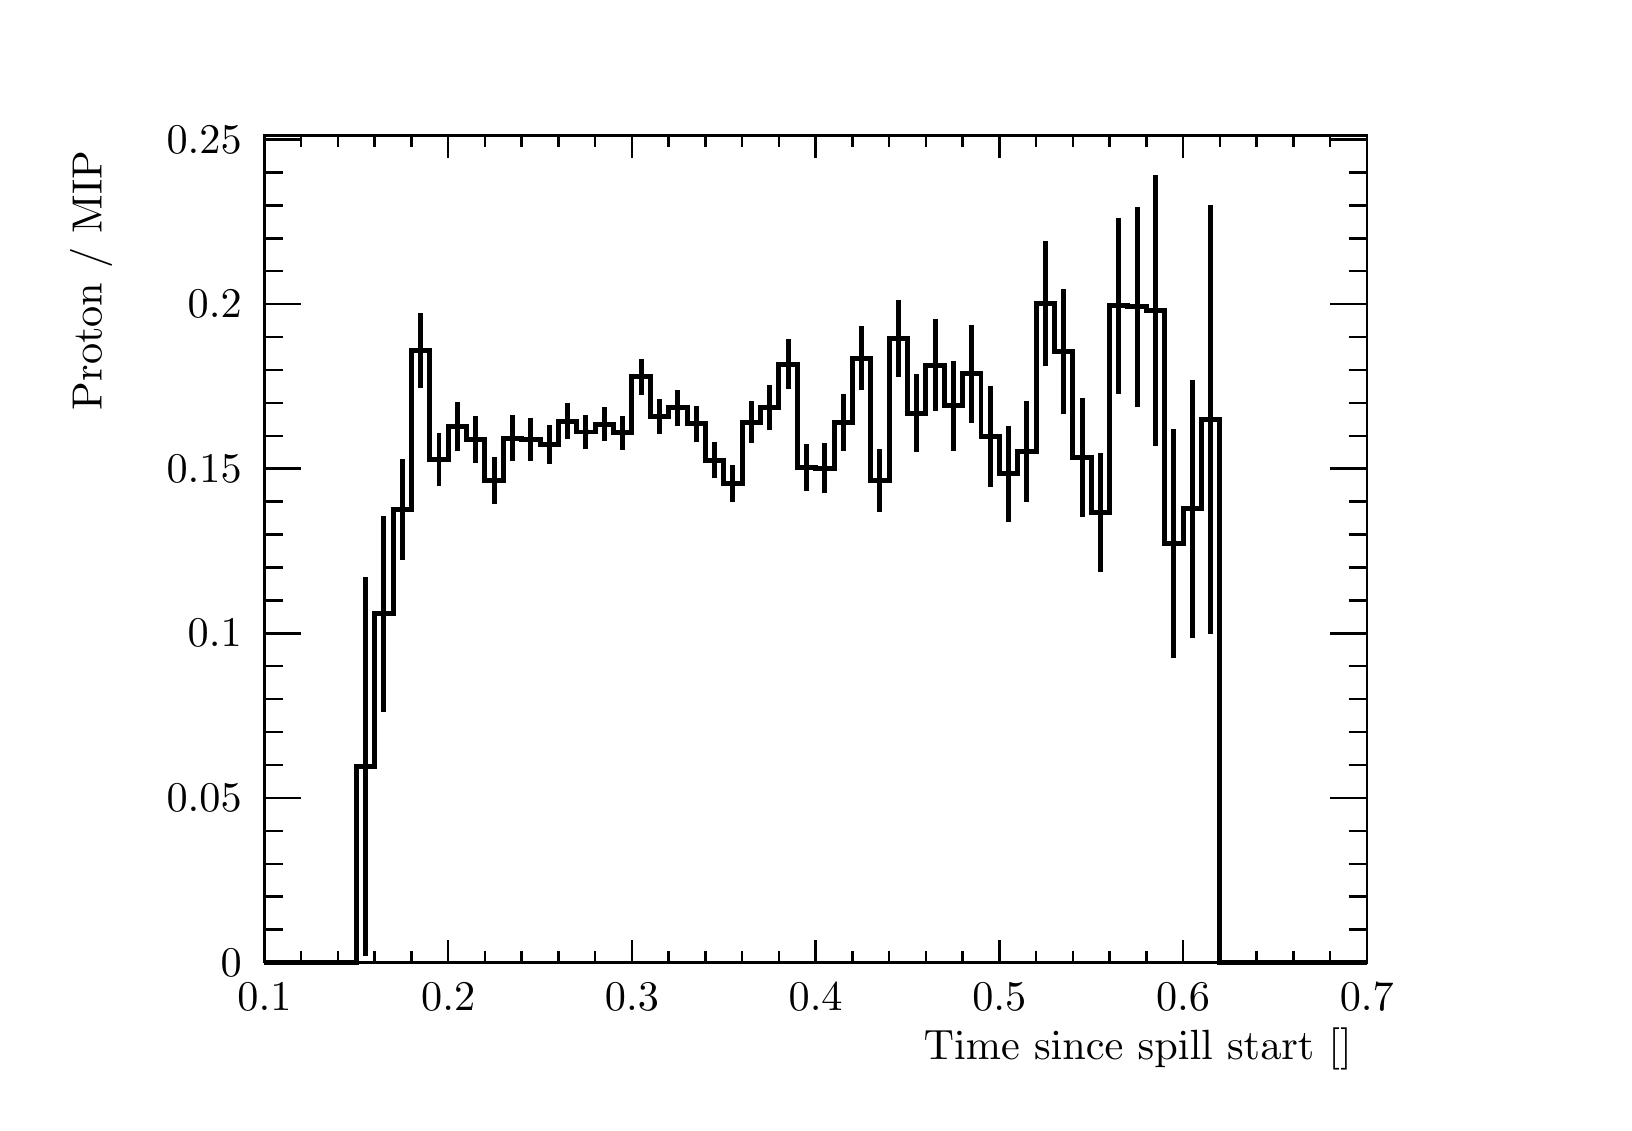
\begin{tikzpicture}
\pgfdeclareplotmark{cross} {
\pgfpathmoveto{\pgfpoint{-0.3\pgfplotmarksize}{\pgfplotmarksize}}
\pgfpathlineto{\pgfpoint{+0.3\pgfplotmarksize}{\pgfplotmarksize}}
\pgfpathlineto{\pgfpoint{+0.3\pgfplotmarksize}{0.3\pgfplotmarksize}}
\pgfpathlineto{\pgfpoint{+1\pgfplotmarksize}{0.3\pgfplotmarksize}}
\pgfpathlineto{\pgfpoint{+1\pgfplotmarksize}{-0.3\pgfplotmarksize}}
\pgfpathlineto{\pgfpoint{+0.3\pgfplotmarksize}{-0.3\pgfplotmarksize}}
\pgfpathlineto{\pgfpoint{+0.3\pgfplotmarksize}{-1.\pgfplotmarksize}}
\pgfpathlineto{\pgfpoint{-0.3\pgfplotmarksize}{-1.\pgfplotmarksize}}
\pgfpathlineto{\pgfpoint{-0.3\pgfplotmarksize}{-0.3\pgfplotmarksize}}
\pgfpathlineto{\pgfpoint{-1.\pgfplotmarksize}{-0.3\pgfplotmarksize}}
\pgfpathlineto{\pgfpoint{-1.\pgfplotmarksize}{0.3\pgfplotmarksize}}
\pgfpathlineto{\pgfpoint{-0.3\pgfplotmarksize}{0.3\pgfplotmarksize}}
\pgfpathclose
\pgfusepathqstroke
}
\pgfdeclareplotmark{cross*} {
\pgfpathmoveto{\pgfpoint{-0.3\pgfplotmarksize}{\pgfplotmarksize}}
\pgfpathlineto{\pgfpoint{+0.3\pgfplotmarksize}{\pgfplotmarksize}}
\pgfpathlineto{\pgfpoint{+0.3\pgfplotmarksize}{0.3\pgfplotmarksize}}
\pgfpathlineto{\pgfpoint{+1\pgfplotmarksize}{0.3\pgfplotmarksize}}
\pgfpathlineto{\pgfpoint{+1\pgfplotmarksize}{-0.3\pgfplotmarksize}}
\pgfpathlineto{\pgfpoint{+0.3\pgfplotmarksize}{-0.3\pgfplotmarksize}}
\pgfpathlineto{\pgfpoint{+0.3\pgfplotmarksize}{-1.\pgfplotmarksize}}
\pgfpathlineto{\pgfpoint{-0.3\pgfplotmarksize}{-1.\pgfplotmarksize}}
\pgfpathlineto{\pgfpoint{-0.3\pgfplotmarksize}{-0.3\pgfplotmarksize}}
\pgfpathlineto{\pgfpoint{-1.\pgfplotmarksize}{-0.3\pgfplotmarksize}}
\pgfpathlineto{\pgfpoint{-1.\pgfplotmarksize}{0.3\pgfplotmarksize}}
\pgfpathlineto{\pgfpoint{-0.3\pgfplotmarksize}{0.3\pgfplotmarksize}}
\pgfpathclose
\pgfusepathqfillstroke
}
\pgfdeclareplotmark{newstar} {
\pgfpathmoveto{\pgfqpoint{0pt}{\pgfplotmarksize}}
\pgfpathlineto{\pgfqpointpolar{44}{0.5\pgfplotmarksize}}
\pgfpathlineto{\pgfqpointpolar{18}{\pgfplotmarksize}}
\pgfpathlineto{\pgfqpointpolar{-20}{0.5\pgfplotmarksize}}
\pgfpathlineto{\pgfqpointpolar{-54}{\pgfplotmarksize}}
\pgfpathlineto{\pgfqpointpolar{-90}{0.5\pgfplotmarksize}}
\pgfpathlineto{\pgfqpointpolar{234}{\pgfplotmarksize}}
\pgfpathlineto{\pgfqpointpolar{198}{0.5\pgfplotmarksize}}
\pgfpathlineto{\pgfqpointpolar{162}{\pgfplotmarksize}}
\pgfpathlineto{\pgfqpointpolar{134}{0.5\pgfplotmarksize}}
\pgfpathclose
\pgfusepathqstroke
}
\pgfdeclareplotmark{newstar*} {
\pgfpathmoveto{\pgfqpoint{0pt}{\pgfplotmarksize}}
\pgfpathlineto{\pgfqpointpolar{44}{0.5\pgfplotmarksize}}
\pgfpathlineto{\pgfqpointpolar{18}{\pgfplotmarksize}}
\pgfpathlineto{\pgfqpointpolar{-20}{0.5\pgfplotmarksize}}
\pgfpathlineto{\pgfqpointpolar{-54}{\pgfplotmarksize}}
\pgfpathlineto{\pgfqpointpolar{-90}{0.5\pgfplotmarksize}}
\pgfpathlineto{\pgfqpointpolar{234}{\pgfplotmarksize}}
\pgfpathlineto{\pgfqpointpolar{198}{0.5\pgfplotmarksize}}
\pgfpathlineto{\pgfqpointpolar{162}{\pgfplotmarksize}}
\pgfpathlineto{\pgfqpointpolar{134}{0.5\pgfplotmarksize}}
\pgfpathclose
\pgfusepathqfillstroke
}
\definecolor{c}{rgb}{1,1,1};
\draw [color=c, fill=c] (0,0) rectangle (20,13.639);
\draw [color=c, fill=c] (3,1.77307) rectangle (17,12.2751);
\definecolor{c}{rgb}{0,0,0};
\draw [c,line width=0.9] (3,1.77307) -- (3,12.2751) -- (17,12.2751) -- (17,1.77307) -- (3,1.77307);
\definecolor{c}{rgb}{1,1,1};
\draw [color=c, fill=c] (3,1.77307) rectangle (17,12.2751);
\definecolor{c}{rgb}{0,0,0};
\draw [c,line width=0.9] (3,1.77307) -- (3,12.2751) -- (17,12.2751) -- (17,1.77307) -- (3,1.77307);
\draw [c,line width=1.8] (4.28333,1.85795) -- (4.28333,4.26597);
\draw [c,line width=1.8] (4.28333,4.26597) -- (4.28333,6.674);
\foreach \P in {(4.28333,4.26597)}{\draw[mark options={color=c,fill=c},mark size=2.402402pt,mark=*,mark size=1pt] plot coordinates {\P};}
\draw [c,line width=1.8] (4.51667,4.95882) -- (4.51667,6.20182);
\draw [c,line width=1.8] (4.51667,6.20182) -- (4.51667,7.44483);
\foreach \P in {(4.51667,6.20182)}{\draw[mark options={color=c,fill=c},mark size=2.402402pt,mark=*,mark size=1pt] plot coordinates {\P};}
\draw [c,line width=1.8] (4.75,6.88558) -- (4.75,7.52999);
\draw [c,line width=1.8] (4.75,7.52999) -- (4.75,8.17441);
\foreach \P in {(4.75,7.52999)}{\draw[mark options={color=c,fill=c},mark size=2.402402pt,mark=*,mark size=1pt] plot coordinates {\P};}
\draw [c,line width=1.8] (4.98333,9.06517) -- (4.98333,9.54667);
\draw [c,line width=1.8] (4.98333,9.54667) -- (4.98333,10.0282);
\foreach \P in {(4.98333,9.54667)}{\draw[mark options={color=c,fill=c},mark size=2.402402pt,mark=*,mark size=1pt] plot coordinates {\P};}
\draw [c,line width=1.8] (5.21667,7.82536) -- (5.21667,8.15941);
\draw [c,line width=1.8] (5.21667,8.15941) -- (5.21667,8.49346);
\foreach \P in {(5.21667,8.15941)}{\draw[mark options={color=c,fill=c},mark size=2.402402pt,mark=*,mark size=1pt] plot coordinates {\P};}
\draw [c,line width=1.8] (5.45,8.26867) -- (5.45,8.57816);
\draw [c,line width=1.8] (5.45,8.57816) -- (5.45,8.88765);
\foreach \P in {(5.45,8.57816)}{\draw[mark options={color=c,fill=c},mark size=2.402402pt,mark=*,mark size=1pt] plot coordinates {\P};}
\draw [c,line width=1.8] (5.68333,8.11213) -- (5.68333,8.41069);
\draw [c,line width=1.8] (5.68333,8.41069) -- (5.68333,8.70926);
\foreach \P in {(5.68333,8.41069)}{\draw[mark options={color=c,fill=c},mark size=2.402402pt,mark=*,mark size=1pt] plot coordinates {\P};}
\draw [c,line width=1.8] (5.91667,7.59665) -- (5.91667,7.89397);
\draw [c,line width=1.8] (5.91667,7.89397) -- (5.91667,8.19129);
\foreach \P in {(5.91667,7.89397)}{\draw[mark options={color=c,fill=c},mark size=2.402402pt,mark=*,mark size=1pt] plot coordinates {\P};}
\draw [c,line width=1.8] (6.15,8.14152) -- (6.15,8.43263);
\draw [c,line width=1.8] (6.15,8.43263) -- (6.15,8.72374);
\foreach \P in {(6.15,8.43263)}{\draw[mark options={color=c,fill=c},mark size=2.402402pt,mark=*,mark size=1pt] plot coordinates {\P};}
\draw [c,line width=1.8] (6.38333,8.14559) -- (6.38333,8.41426);
\draw [c,line width=1.8] (6.38333,8.41426) -- (6.38333,8.68294);
\foreach \P in {(6.38333,8.41426)}{\draw[mark options={color=c,fill=c},mark size=2.402402pt,mark=*,mark size=1pt] plot coordinates {\P};}
\draw [c,line width=1.8] (6.61667,8.09959) -- (6.61667,8.34791);
\draw [c,line width=1.8] (6.61667,8.34791) -- (6.61667,8.59622);
\foreach \P in {(6.61667,8.34791)}{\draw[mark options={color=c,fill=c},mark size=2.402402pt,mark=*,mark size=1pt] plot coordinates {\P};}
\draw [c,line width=1.8] (6.85,8.41637) -- (6.85,8.64916);
\draw [c,line width=1.8] (6.85,8.64916) -- (6.85,8.88195);
\foreach \P in {(6.85,8.64916)}{\draw[mark options={color=c,fill=c},mark size=2.402402pt,mark=*,mark size=1pt] plot coordinates {\P};}
\draw [c,line width=1.8] (7.08333,8.28923) -- (7.08333,8.51105);
\draw [c,line width=1.8] (7.08333,8.51105) -- (7.08333,8.73287);
\foreach \P in {(7.08333,8.51105)}{\draw[mark options={color=c,fill=c},mark size=2.402402pt,mark=*,mark size=1pt] plot coordinates {\P};}
\draw [c,line width=1.8] (7.31667,8.39124) -- (7.31667,8.60961);
\draw [c,line width=1.8] (7.31667,8.60961) -- (7.31667,8.82799);
\foreach \P in {(7.31667,8.60961)}{\draw[mark options={color=c,fill=c},mark size=2.402402pt,mark=*,mark size=1pt] plot coordinates {\P};}
\draw [c,line width=1.8] (7.55,8.28584) -- (7.55,8.49863);
\draw [c,line width=1.8] (7.55,8.49863) -- (7.55,8.71142);
\foreach \P in {(7.55,8.49863)}{\draw[mark options={color=c,fill=c},mark size=2.402402pt,mark=*,mark size=1pt] plot coordinates {\P};}
\draw [c,line width=1.8] (7.78333,8.98351) -- (7.78333,9.21265);
\draw [c,line width=1.8] (7.78333,9.21265) -- (7.78333,9.44178);
\foreach \P in {(7.78333,9.21265)}{\draw[mark options={color=c,fill=c},mark size=2.402402pt,mark=*,mark size=1pt] plot coordinates {\P};}
\draw [c,line width=1.8] (8.01667,8.47948) -- (8.01667,8.70265);
\draw [c,line width=1.8] (8.01667,8.70265) -- (8.01667,8.92583);
\foreach \P in {(8.01667,8.70265)}{\draw[mark options={color=c,fill=c},mark size=2.402402pt,mark=*,mark size=1pt] plot coordinates {\P};}
\draw [c,line width=1.8] (8.25,8.58929) -- (8.25,8.81786);
\draw [c,line width=1.8] (8.25,8.81786) -- (8.25,9.04643);
\foreach \P in {(8.25,8.81786)}{\draw[mark options={color=c,fill=c},mark size=2.402402pt,mark=*,mark size=1pt] plot coordinates {\P};}
\draw [c,line width=1.8] (8.48333,8.38024) -- (8.48333,8.61365);
\draw [c,line width=1.8] (8.48333,8.61365) -- (8.48333,8.84705);
\foreach \P in {(8.48333,8.61365)}{\draw[mark options={color=c,fill=c},mark size=2.402402pt,mark=*,mark size=1pt] plot coordinates {\P};}
\draw [c,line width=1.8] (8.71667,7.9206) -- (8.71667,8.15484);
\draw [c,line width=1.8] (8.71667,8.15484) -- (8.71667,8.38908);
\foreach \P in {(8.71667,8.15484)}{\draw[mark options={color=c,fill=c},mark size=2.402402pt,mark=*,mark size=1pt] plot coordinates {\P};}
\draw [c,line width=1.8] (8.95,7.62004) -- (8.95,7.85569);
\draw [c,line width=1.8] (8.95,7.85569) -- (8.95,8.09134);
\foreach \P in {(8.95,7.85569)}{\draw[mark options={color=c,fill=c},mark size=2.402402pt,mark=*,mark size=1pt] plot coordinates {\P};}
\draw [c,line width=1.8] (9.18333,8.36926) -- (9.18333,8.63709);
\draw [c,line width=1.8] (9.18333,8.63709) -- (9.18333,8.90492);
\foreach \P in {(9.18333,8.63709)}{\draw[mark options={color=c,fill=c},mark size=2.402402pt,mark=*,mark size=1pt] plot coordinates {\P};}
\draw [c,line width=1.8] (9.41667,8.53941) -- (9.41667,8.82537);
\draw [c,line width=1.8] (9.41667,8.82537) -- (9.41667,9.11132);
\foreach \P in {(9.41667,8.82537)}{\draw[mark options={color=c,fill=c},mark size=2.402402pt,mark=*,mark size=1pt] plot coordinates {\P};}
\draw [c,line width=1.8] (9.65,9.05386) -- (9.65,9.36986);
\draw [c,line width=1.8] (9.65,9.36986) -- (9.65,9.68587);
\foreach \P in {(9.65,9.36986)}{\draw[mark options={color=c,fill=c},mark size=2.402402pt,mark=*,mark size=1pt] plot coordinates {\P};}
\draw [c,line width=1.8] (9.88333,7.76146) -- (9.88333,8.06142);
\draw [c,line width=1.8] (9.88333,8.06142) -- (9.88333,8.36138);
\foreach \P in {(9.88333,8.06142)}{\draw[mark options={color=c,fill=c},mark size=2.402402pt,mark=*,mark size=1pt] plot coordinates {\P};}
\draw [c,line width=1.8] (10.1167,7.73575) -- (10.1167,8.05126);
\draw [c,line width=1.8] (10.1167,8.05126) -- (10.1167,8.36676);
\foreach \P in {(10.1167,8.05126)}{\draw[mark options={color=c,fill=c},mark size=2.402402pt,mark=*,mark size=1pt] plot coordinates {\P};}
\draw [c,line width=1.8] (10.35,8.2671) -- (10.35,8.63019);
\draw [c,line width=1.8] (10.35,8.63019) -- (10.35,8.99327);
\foreach \P in {(10.35,8.63019)}{\draw[mark options={color=c,fill=c},mark size=2.402402pt,mark=*,mark size=1pt] plot coordinates {\P};}
\draw [c,line width=1.8] (10.5833,9.04507) -- (10.5833,9.44879);
\draw [c,line width=1.8] (10.5833,9.44879) -- (10.5833,9.85251);
\foreach \P in {(10.5833,9.44879)}{\draw[mark options={color=c,fill=c},mark size=2.402402pt,mark=*,mark size=1pt] plot coordinates {\P};}
\draw [c,line width=1.8] (10.8167,7.50104) -- (10.8167,7.89536);
\draw [c,line width=1.8] (10.8167,7.89536) -- (10.8167,8.28967);
\foreach \P in {(10.8167,7.89536)}{\draw[mark options={color=c,fill=c},mark size=2.402402pt,mark=*,mark size=1pt] plot coordinates {\P};}
\draw [c,line width=1.8] (11.05,9.21278) -- (11.05,9.7027);
\draw [c,line width=1.8] (11.05,9.7027) -- (11.05,10.1926);
\foreach \P in {(11.05,9.7027)}{\draw[mark options={color=c,fill=c},mark size=2.402402pt,mark=*,mark size=1pt] plot coordinates {\P};}
\draw [c,line width=1.8] (11.2833,8.25238) -- (11.2833,8.74718);
\draw [c,line width=1.8] (11.2833,8.74718) -- (11.2833,9.24198);
\foreach \P in {(11.2833,8.74718)}{\draw[mark options={color=c,fill=c},mark size=2.402402pt,mark=*,mark size=1pt] plot coordinates {\P};}
\draw [c,line width=1.8] (11.5167,8.77527) -- (11.5167,9.35802);
\draw [c,line width=1.8] (11.5167,9.35802) -- (11.5167,9.94076);
\foreach \P in {(11.5167,9.35802)}{\draw[mark options={color=c,fill=c},mark size=2.402402pt,mark=*,mark size=1pt] plot coordinates {\P};}
\draw [c,line width=1.8] (11.75,8.27462) -- (11.75,8.84624);
\draw [c,line width=1.8] (11.75,8.84624) -- (11.75,9.41786);
\foreach \P in {(11.75,8.84624)}{\draw[mark options={color=c,fill=c},mark size=2.402402pt,mark=*,mark size=1pt] plot coordinates {\P};}
\draw [c,line width=1.8] (11.9833,8.63141) -- (11.9833,9.2513);
\draw [c,line width=1.8] (11.9833,9.2513) -- (11.9833,9.8712);
\foreach \P in {(11.9833,9.2513)}{\draw[mark options={color=c,fill=c},mark size=2.402402pt,mark=*,mark size=1pt] plot coordinates {\P};}
\draw [c,line width=1.8] (12.2167,7.81775) -- (12.2167,8.45422);
\draw [c,line width=1.8] (12.2167,8.45422) -- (12.2167,9.09069);
\foreach \P in {(12.2167,8.45422)}{\draw[mark options={color=c,fill=c},mark size=2.402402pt,mark=*,mark size=1pt] plot coordinates {\P};}
\draw [c,line width=1.8] (12.45,7.36943) -- (12.45,7.97822);
\draw [c,line width=1.8] (12.45,7.97822) -- (12.45,8.58701);
\foreach \P in {(12.45,7.97822)}{\draw[mark options={color=c,fill=c},mark size=2.402402pt,mark=*,mark size=1pt] plot coordinates {\P};}
\draw [c,line width=1.8] (12.6833,7.61971) -- (12.6833,8.26531);
\draw [c,line width=1.8] (12.6833,8.26531) -- (12.6833,8.91091);
\foreach \P in {(12.6833,8.26531)}{\draw[mark options={color=c,fill=c},mark size=2.402402pt,mark=*,mark size=1pt] plot coordinates {\P};}
\draw [c,line width=1.8] (12.9167,9.34774) -- (12.9167,10.144);
\draw [c,line width=1.8] (12.9167,10.144) -- (12.9167,10.9402);
\foreach \P in {(12.9167,10.144)}{\draw[mark options={color=c,fill=c},mark size=2.402402pt,mark=*,mark size=1pt] plot coordinates {\P};}
\draw [c,line width=1.8] (13.15,8.74157) -- (13.15,9.53696);
\draw [c,line width=1.8] (13.15,9.53696) -- (13.15,10.3324);
\foreach \P in {(13.15,9.53696)}{\draw[mark options={color=c,fill=c},mark size=2.402402pt,mark=*,mark size=1pt] plot coordinates {\P};}
\draw [c,line width=1.8] (13.3833,7.43321) -- (13.3833,8.1871);
\draw [c,line width=1.8] (13.3833,8.1871) -- (13.3833,8.941);
\foreach \P in {(13.3833,8.1871)}{\draw[mark options={color=c,fill=c},mark size=2.402402pt,mark=*,mark size=1pt] plot coordinates {\P};}
\draw [c,line width=1.8] (13.6167,6.72893) -- (13.6167,7.48532);
\draw [c,line width=1.8] (13.6167,7.48532) -- (13.6167,8.2417);
\foreach \P in {(13.6167,7.48532)}{\draw[mark options={color=c,fill=c},mark size=2.402402pt,mark=*,mark size=1pt] plot coordinates {\P};}
\draw [c,line width=1.8] (13.85,8.99665) -- (13.85,10.1133);
\draw [c,line width=1.8] (13.85,10.1133) -- (13.85,11.2299);
\foreach \P in {(13.85,10.1133)}{\draw[mark options={color=c,fill=c},mark size=2.402402pt,mark=*,mark size=1pt] plot coordinates {\P};}
\draw [c,line width=1.8] (14.0833,8.83049) -- (14.0833,10.1011);
\draw [c,line width=1.8] (14.0833,10.1011) -- (14.0833,11.3716);
\foreach \P in {(14.0833,10.1011)}{\draw[mark options={color=c,fill=c},mark size=2.402402pt,mark=*,mark size=1pt] plot coordinates {\P};}
\draw [c,line width=1.8] (14.3167,8.33544) -- (14.3167,10.0552);
\draw [c,line width=1.8] (14.3167,10.0552) -- (14.3167,11.775);
\foreach \P in {(14.3167,10.0552)}{\draw[mark options={color=c,fill=c},mark size=2.402402pt,mark=*,mark size=1pt] plot coordinates {\P};}
\draw [c,line width=1.8] (14.55,5.64668) -- (14.55,7.09824);
\draw [c,line width=1.8] (14.55,7.09824) -- (14.55,8.5498);
\foreach \P in {(14.55,7.09824)}{\draw[mark options={color=c,fill=c},mark size=2.402402pt,mark=*,mark size=1pt] plot coordinates {\P};}
\draw [c,line width=1.8] (14.7833,5.89349) -- (14.7833,7.53431);
\draw [c,line width=1.8] (14.7833,7.53431) -- (14.7833,9.17514);
\foreach \P in {(14.7833,7.53431)}{\draw[mark options={color=c,fill=c},mark size=2.402402pt,mark=*,mark size=1pt] plot coordinates {\P};}
\draw [c,line width=1.8] (15.0167,5.94687) -- (15.0167,8.6719);
\draw [c,line width=1.8] (15.0167,8.6719) -- (15.0167,11.3969);
\foreach \P in {(15.0167,8.6719)}{\draw[mark options={color=c,fill=c},mark size=2.402402pt,mark=*,mark size=1pt] plot coordinates {\P};}
\draw [c,line width=1.8] (3,1.77307) -- (3.23333,1.77307) -- (3.23333,1.77307) -- (3.46667,1.77307) -- (3.46667,1.77307) -- (3.7,1.77307) -- (3.7,1.77307) -- (3.93333,1.77307) -- (3.93333,1.77307) -- (4.16667,1.77307) -- (4.16667,4.26597) --
 (4.4,4.26597) -- (4.4,6.20182) -- (4.63333,6.20182) -- (4.63333,7.52999) -- (4.86667,7.52999) -- (4.86667,9.54667) -- (5.1,9.54667) -- (5.1,8.15941) -- (5.33333,8.15941) -- (5.33333,8.57816) -- (5.56667,8.57816) -- (5.56667,8.41069) -- (5.8,8.41069)
 -- (5.8,7.89397) -- (6.03333,7.89397) -- (6.03333,8.43263) -- (6.26667,8.43263) -- (6.26667,8.41426) -- (6.5,8.41426) -- (6.5,8.34791) -- (6.73333,8.34791) -- (6.73333,8.64916) -- (6.96667,8.64916) -- (6.96667,8.51105) -- (7.2,8.51105) --
 (7.2,8.60961) -- (7.43333,8.60961) -- (7.43333,8.49863) -- (7.66667,8.49863) -- (7.66667,9.21265) -- (7.9,9.21265) -- (7.9,8.70265) -- (8.13333,8.70265) -- (8.13333,8.81786) -- (8.36667,8.81786) -- (8.36667,8.61365) -- (8.6,8.61365) -- (8.6,8.15484)
 -- (8.83333,8.15484) -- (8.83333,7.85569) -- (9.06667,7.85569) -- (9.06667,8.63709) -- (9.3,8.63709) -- (9.3,8.82537) -- (9.53333,8.82537) -- (9.53333,9.36986) -- (9.76667,9.36986) -- (9.76667,8.06142) -- (10,8.06142) -- (10,8.05126) --
 (10.2333,8.05126) -- (10.2333,8.63019) -- (10.4667,8.63019) -- (10.4667,9.44879) -- (10.7,9.44879) -- (10.7,7.89536) -- (10.9333,7.89536) -- (10.9333,9.7027) -- (11.1667,9.7027) -- (11.1667,8.74718) -- (11.4,8.74718) -- (11.4,9.35802) --
 (11.6333,9.35802) -- (11.6333,8.84624) -- (11.8667,8.84624) -- (11.8667,9.2513) -- (12.1,9.2513) -- (12.1,8.45422) -- (12.3333,8.45422) -- (12.3333,7.97822) -- (12.5667,7.97822) -- (12.5667,8.26531) -- (12.8,8.26531) -- (12.8,10.144) --
 (13.0333,10.144) -- (13.0333,9.53696) -- (13.2667,9.53696) -- (13.2667,8.1871) -- (13.5,8.1871) -- (13.5,7.48532) -- (13.7333,7.48532) -- (13.7333,10.1133) -- (13.9667,10.1133) -- (13.9667,10.1011) -- (14.2,10.1011) -- (14.2,10.0552) --
 (14.4333,10.0552) -- (14.4333,7.09824) -- (14.6667,7.09824) -- (14.6667,7.53431) -- (14.9,7.53431) -- (14.9,8.6719) -- (15.1333,8.6719) -- (15.1333,1.77307) -- (15.3667,1.77307) -- (15.3667,1.77307) -- (15.6,1.77307) -- (15.6,1.77307) --
 (15.8333,1.77307) -- (15.8333,1.77307) -- (16.0667,1.77307) -- (16.0667,1.77307) -- (16.3,1.77307) -- (16.3,1.77307) -- (16.5333,1.77307) -- (16.5333,1.77307) -- (16.7667,1.77307) -- (16.7667,1.77307) -- (17,1.77307);
\draw [c,line width=0.9] (3,1.77307) -- (17,1.77307);
\draw [c,line width=0.9] (3,2.05948) -- (3,1.77307);
\draw [c,line width=0.9] (3.46667,1.91628) -- (3.46667,1.77307);
\draw [c,line width=0.9] (3.93333,1.91628) -- (3.93333,1.77307);
\draw [c,line width=0.9] (4.4,1.91628) -- (4.4,1.77307);
\draw [c,line width=0.9] (4.86667,1.91628) -- (4.86667,1.77307);
\draw [c,line width=0.9] (5.33333,2.05948) -- (5.33333,1.77307);
\draw [c,line width=0.9] (5.8,1.91628) -- (5.8,1.77307);
\draw [c,line width=0.9] (6.26667,1.91628) -- (6.26667,1.77307);
\draw [c,line width=0.9] (6.73333,1.91628) -- (6.73333,1.77307);
\draw [c,line width=0.9] (7.2,1.91628) -- (7.2,1.77307);
\draw [c,line width=0.9] (7.66667,2.05948) -- (7.66667,1.77307);
\draw [c,line width=0.9] (8.13333,1.91628) -- (8.13333,1.77307);
\draw [c,line width=0.9] (8.6,1.91628) -- (8.6,1.77307);
\draw [c,line width=0.9] (9.06667,1.91628) -- (9.06667,1.77307);
\draw [c,line width=0.9] (9.53333,1.91628) -- (9.53333,1.77307);
\draw [c,line width=0.9] (10,2.05948) -- (10,1.77307);
\draw [c,line width=0.9] (10.4667,1.91628) -- (10.4667,1.77307);
\draw [c,line width=0.9] (10.9333,1.91628) -- (10.9333,1.77307);
\draw [c,line width=0.9] (11.4,1.91628) -- (11.4,1.77307);
\draw [c,line width=0.9] (11.8667,1.91628) -- (11.8667,1.77307);
\draw [c,line width=0.9] (12.3333,2.05948) -- (12.3333,1.77307);
\draw [c,line width=0.9] (12.8,1.91628) -- (12.8,1.77307);
\draw [c,line width=0.9] (13.2667,1.91628) -- (13.2667,1.77307);
\draw [c,line width=0.9] (13.7333,1.91628) -- (13.7333,1.77307);
\draw [c,line width=0.9] (14.2,1.91628) -- (14.2,1.77307);
\draw [c,line width=0.9] (14.6667,2.05948) -- (14.6667,1.77307);
\draw [c,line width=0.9] (15.1333,1.91628) -- (15.1333,1.77307);
\draw [c,line width=0.9] (15.6,1.91628) -- (15.6,1.77307);
\draw [c,line width=0.9] (16.0667,1.91628) -- (16.0667,1.77307);
\draw [c,line width=0.9] (16.5333,1.91628) -- (16.5333,1.77307);
\draw [c,line width=0.9] (17,2.05948) -- (17,1.77307);
\draw [c,line width=0.9] (17,2.05948) -- (17,1.77307);
\draw [anchor=base] (3,1.15931) node[scale=1.52731, color=c, rotate=0]{0.1};
\draw [anchor=base] (5.33333,1.15931) node[scale=1.52731, color=c, rotate=0]{0.2};
\draw [anchor=base] (7.66667,1.15931) node[scale=1.52731, color=c, rotate=0]{0.3};
\draw [anchor=base] (10,1.15931) node[scale=1.52731, color=c, rotate=0]{0.4};
\draw [anchor=base] (12.3333,1.15931) node[scale=1.52731, color=c, rotate=0]{0.5};
\draw [anchor=base] (14.6667,1.15931) node[scale=1.52731, color=c, rotate=0]{0.6};
\draw [anchor=base] (17,1.15931) node[scale=1.52731, color=c, rotate=0]{0.7};
\draw [anchor= east] (17,0.681948) node[scale=1.52731, color=c, rotate=0]{ Time since spill start [\si{\nano\second}]};
\draw [c,line width=0.9] (3,12.2751) -- (17,12.2751);
\draw [c,line width=0.9] (3,11.9887) -- (3,12.2751);
\draw [c,line width=0.9] (3.46667,12.1319) -- (3.46667,12.2751);
\draw [c,line width=0.9] (3.93333,12.1319) -- (3.93333,12.2751);
\draw [c,line width=0.9] (4.4,12.1319) -- (4.4,12.2751);
\draw [c,line width=0.9] (4.86667,12.1319) -- (4.86667,12.2751);
\draw [c,line width=0.9] (5.33333,11.9887) -- (5.33333,12.2751);
\draw [c,line width=0.9] (5.8,12.1319) -- (5.8,12.2751);
\draw [c,line width=0.9] (6.26667,12.1319) -- (6.26667,12.2751);
\draw [c,line width=0.9] (6.73333,12.1319) -- (6.73333,12.2751);
\draw [c,line width=0.9] (7.2,12.1319) -- (7.2,12.2751);
\draw [c,line width=0.9] (7.66667,11.9887) -- (7.66667,12.2751);
\draw [c,line width=0.9] (8.13333,12.1319) -- (8.13333,12.2751);
\draw [c,line width=0.9] (8.6,12.1319) -- (8.6,12.2751);
\draw [c,line width=0.9] (9.06667,12.1319) -- (9.06667,12.2751);
\draw [c,line width=0.9] (9.53333,12.1319) -- (9.53333,12.2751);
\draw [c,line width=0.9] (10,11.9887) -- (10,12.2751);
\draw [c,line width=0.9] (10.4667,12.1319) -- (10.4667,12.2751);
\draw [c,line width=0.9] (10.9333,12.1319) -- (10.9333,12.2751);
\draw [c,line width=0.9] (11.4,12.1319) -- (11.4,12.2751);
\draw [c,line width=0.9] (11.8667,12.1319) -- (11.8667,12.2751);
\draw [c,line width=0.9] (12.3333,11.9887) -- (12.3333,12.2751);
\draw [c,line width=0.9] (12.8,12.1319) -- (12.8,12.2751);
\draw [c,line width=0.9] (13.2667,12.1319) -- (13.2667,12.2751);
\draw [c,line width=0.9] (13.7333,12.1319) -- (13.7333,12.2751);
\draw [c,line width=0.9] (14.2,12.1319) -- (14.2,12.2751);
\draw [c,line width=0.9] (14.6667,11.9887) -- (14.6667,12.2751);
\draw [c,line width=0.9] (15.1333,12.1319) -- (15.1333,12.2751);
\draw [c,line width=0.9] (15.6,12.1319) -- (15.6,12.2751);
\draw [c,line width=0.9] (16.0667,12.1319) -- (16.0667,12.2751);
\draw [c,line width=0.9] (16.5333,12.1319) -- (16.5333,12.2751);
\draw [c,line width=0.9] (17,11.9887) -- (17,12.2751);
\draw [c,line width=0.9] (17,11.9887) -- (17,12.2751);
\draw [c,line width=0.9] (3,1.77307) -- (3,12.2751);
\draw [c,line width=0.9] (3.462,1.77307) -- (3,1.77307);
\draw [c,line width=0.9] (3.231,2.19118) -- (3,2.19118);
\draw [c,line width=0.9] (3.231,2.60929) -- (3,2.60929);
\draw [c,line width=0.9] (3.231,3.0274) -- (3,3.0274);
\draw [c,line width=0.9] (3.231,3.44551) -- (3,3.44551);
\draw [c,line width=0.9] (3.462,3.86362) -- (3,3.86362);
\draw [c,line width=0.9] (3.231,4.28173) -- (3,4.28173);
\draw [c,line width=0.9] (3.231,4.69984) -- (3,4.69984);
\draw [c,line width=0.9] (3.231,5.11795) -- (3,5.11795);
\draw [c,line width=0.9] (3.231,5.53606) -- (3,5.53606);
\draw [c,line width=0.9] (3.462,5.95417) -- (3,5.95417);
\draw [c,line width=0.9] (3.231,6.37228) -- (3,6.37228);
\draw [c,line width=0.9] (3.231,6.79039) -- (3,6.79039);
\draw [c,line width=0.9] (3.231,7.2085) -- (3,7.2085);
\draw [c,line width=0.9] (3.231,7.62661) -- (3,7.62661);
\draw [c,line width=0.9] (3.462,8.04472) -- (3,8.04472);
\draw [c,line width=0.9] (3.231,8.46283) -- (3,8.46283);
\draw [c,line width=0.9] (3.231,8.88094) -- (3,8.88094);
\draw [c,line width=0.9] (3.231,9.29905) -- (3,9.29905);
\draw [c,line width=0.9] (3.231,9.71716) -- (3,9.71716);
\draw [c,line width=0.9] (3.462,10.1353) -- (3,10.1353);
\draw [c,line width=0.9] (3.231,10.5534) -- (3,10.5534);
\draw [c,line width=0.9] (3.231,10.9715) -- (3,10.9715);
\draw [c,line width=0.9] (3.231,11.3896) -- (3,11.3896);
\draw [c,line width=0.9] (3.231,11.8077) -- (3,11.8077);
\draw [c,line width=0.9] (3.462,12.2258) -- (3,12.2258);
\draw [c,line width=0.9] (3.462,12.2258) -- (3,12.2258);
\draw [anchor= east] (2.9,1.77307) node[scale=1.52731, color=c, rotate=0]{0};
\draw [anchor= east] (2.9,3.86362) node[scale=1.52731, color=c, rotate=0]{0.05};
\draw [anchor= east] (2.9,5.95417) node[scale=1.52731, color=c, rotate=0]{0.1};
\draw [anchor= east] (2.9,8.04472) node[scale=1.52731, color=c, rotate=0]{0.15};
\draw [anchor= east] (2.9,10.1353) node[scale=1.52731, color=c, rotate=0]{0.2};
\draw [anchor= east] (2.9,12.2258) node[scale=1.52731, color=c, rotate=0]{0.25};
\draw [anchor= east] (0.796562,12.2751) node[scale=1.52731, color=c, rotate=90]{ Proton / MIP};
\draw [c,line width=0.9] (17,1.77307) -- (17,12.2751);
\draw [c,line width=0.9] (16.538,1.77307) -- (17,1.77307);
\draw [c,line width=0.9] (16.769,2.19118) -- (17,2.19118);
\draw [c,line width=0.9] (16.769,2.60929) -- (17,2.60929);
\draw [c,line width=0.9] (16.769,3.0274) -- (17,3.0274);
\draw [c,line width=0.9] (16.769,3.44551) -- (17,3.44551);
\draw [c,line width=0.9] (16.538,3.86362) -- (17,3.86362);
\draw [c,line width=0.9] (16.769,4.28173) -- (17,4.28173);
\draw [c,line width=0.9] (16.769,4.69984) -- (17,4.69984);
\draw [c,line width=0.9] (16.769,5.11795) -- (17,5.11795);
\draw [c,line width=0.9] (16.769,5.53606) -- (17,5.53606);
\draw [c,line width=0.9] (16.538,5.95417) -- (17,5.95417);
\draw [c,line width=0.9] (16.769,6.37228) -- (17,6.37228);
\draw [c,line width=0.9] (16.769,6.79039) -- (17,6.79039);
\draw [c,line width=0.9] (16.769,7.2085) -- (17,7.2085);
\draw [c,line width=0.9] (16.769,7.62661) -- (17,7.62661);
\draw [c,line width=0.9] (16.538,8.04472) -- (17,8.04472);
\draw [c,line width=0.9] (16.769,8.46283) -- (17,8.46283);
\draw [c,line width=0.9] (16.769,8.88094) -- (17,8.88094);
\draw [c,line width=0.9] (16.769,9.29905) -- (17,9.29905);
\draw [c,line width=0.9] (16.769,9.71716) -- (17,9.71716);
\draw [c,line width=0.9] (16.538,10.1353) -- (17,10.1353);
\draw [c,line width=0.9] (16.769,10.5534) -- (17,10.5534);
\draw [c,line width=0.9] (16.769,10.9715) -- (17,10.9715);
\draw [c,line width=0.9] (16.769,11.3896) -- (17,11.3896);
\draw [c,line width=0.9] (16.769,11.8077) -- (17,11.8077);
\draw [c,line width=0.9] (16.538,12.2258) -- (17,12.2258);
\draw [c,line width=0.9] (16.538,12.2258) -- (17,12.2258);
\definecolor{c}{rgb}{1,1,1};
\draw [color=c, fill=c] (2,12.8206) rectangle (18,13.5708);
\definecolor{c}{rgb}{0,0,0};
%\draw (10,13.1957) node[scale=1.40004, color=c, rotate=0]{2 blocks: Proton/MIP};
\end{tikzpicture}
